%%%%%%%%%%%%%%%%%%%%%%%%%%%%%%%%%%%%%%%%%
% University/School Laboratory Report
% LaTeX Template
% Version 3.1 (25/3/14)
%
% This template has been downloaded from:
% http://www.LaTeXTemplates.com
%
% Original author:
% Linux and Unix Users Group at Virginia Tech Wiki
% (https://vtluug.org/wiki/Example_LaTeX_chem_lab_report)
%
% License:
% CC BY-NC-SA 3.0 (http://creativecommons.org/licenses/by-nc-sa/3.0/)
%
%%%%%%%%%%%%%%%%%%%%%%%%%%%%%%%%%%%%%%%%%

%----------------------------------------------------------------------------------------
%	PACKAGES AND DOCUMENT CONFIGURATIONS
%----------------------------------------------------------------------------------------

\documentclass{article}

\usepackage[brazil]{babel}
\usepackage[utf8]{inputenc}
\usepackage[T1]{fontenc}
\usepackage{graphicx} % Required for the inclusion of images
\usepackage{float}

\setlength\parindent{0pt} % Removes all indentation from paragraphs

\renewcommand{\labelenumi}{\alph{enumi}.} % Make numbering in the enumerate environment by letter rather than number (e.g. section 6)

%\usepackage{times} % Uncomment to use the Times New Roman font

%----------------------------------------------------------------------------------------
%	DOCUMENT INFORMATION
%----------------------------------------------------------------------------------------

\title{Implementação do Tetris \\ em MIPS Assembly \\ Utilizando Simulador MARS} % Title

\author{Jonathas Conceição \\ Lucas Bretana} % Author name

\date{\today} % Date for the report

\begin{document}

\maketitle % Insert the title, author and date

\begin{center}
\begin{tabular}{l r}
Data da Entrega: & 08, Julho, 2016 \\ % Date the experiment was performed
\end{tabular}
\end{center}

% If you wish to include an abstract, uncomment the lines below
% \begin{abstract}
% Abstract text
% \end{abstract}

%----------------------------------------------------------------------------------------
%	SECTION 1
%----------------------------------------------------------------------------------------

\section{Objetivo}

Implementar o clássico jogo russo da década de 80, \textit{Tetris}, em MIPS Assembly utilizando o simulador MARS(\textit{MIPS Assembler and Runtime Simulator}).

% To determine the atomic weight of magnesium via its reaction with oxygen and to study the stoichiometry of the reaction (as defined in \ref{definitions}):

% \begin{center}\ce{2 Mg + O2 -> 2 MgO}\end{center}

% If you have more than one objective, uncomment the below:
%\begin{description}
%\item[First Objective] \hfill \\
%Objective 1 text
%\item[Second Objective] \hfill \\
%Objective 2 text
%\end{description}

\subsection{Definições} \label{definitions}
\begin{description}
  \item[Interface:]
    É proposto a implementação uma interface gráfica utilizando o Bitmap Dispaly do MARS, possuindo em sua interface a área de jogo, bem como pontuação, linhas completadas e próxima peça.
  \item[Menu:]
    Possuir um menu básico de interação com usuário permitindo começar uma nova partida ou sair do jogo.
  \item[Movimentação:]
    Permitir a movimentação e rotação das peças por meio de uma leitura do teclado utilizando a ferramenta de \textit{Memory-Mapped I/O} presente no MARS.
\end{description}

%----------------------------------------------------------------------------------------
%	SECTION 2
%----------------------------------------------------------------------------------------

\section{Recursos Utilizados}

Para este projeto foram utilizados os seguintes recursos presentes no MARS:
\begin{itemize}
  \item \textbf{Macros}, utilizado para simplificar a codificação do projeto.
  \item \textbf{Bitmap Display}, para interface gráfica.
  \item \textbf{Keyboard and Display MMIO Simulator}, para leitura das ações do usuário.
  \item \textbf{Pseudo Instruções}, para simplificar a codificação do projeto.
  \item \textbf{Tratamento de Exceções}, para gerar uma peça aleatória e para finilizar a simulação.
  % \item \textbf{Aseprite}, software open source de pixel-art para auxiliar desenho da interface gráfica.
  % \item \textbf{}, .
\end{itemize}

%----------------------------------------------------------------------------------------
%	SECTION 3
%----------------------------------------------------------------------------------------

\section{Metodologia}

Primeiramente foi desenvolvido uma série de macros relacionados a interface gráfica para simplificar o desenho da interface bem como das peças na tela e a aritmética para movimentação dos ponteiros.

Fez-se necessário a implementação de uma outra estrutura de dados além da pilha, uma fila para armazenamento de dados para a movimentação das peças.

Junto aos macros foram utilizados também sobrotinas(funções) mas deixar o código mais claro. As subrotinas possuem uma nomenclatura mais direta a cerca do que é feito no código, e esta por sua vez chama os macros necessários para sua execução.

A interface possui um tamanho de 512x512 pixels. Para simplificar o desenho e a movimentação do ponteiro foi convencionado uma divisão da tela de 32x32 blocos com 16x16 pixels cada.

%----------------------------------------------------------------------------------------
%	SECTION 4
%----------------------------------------------------------------------------------------

\section{Resultados}

\begin{figure}[H]
  \begin{center}
    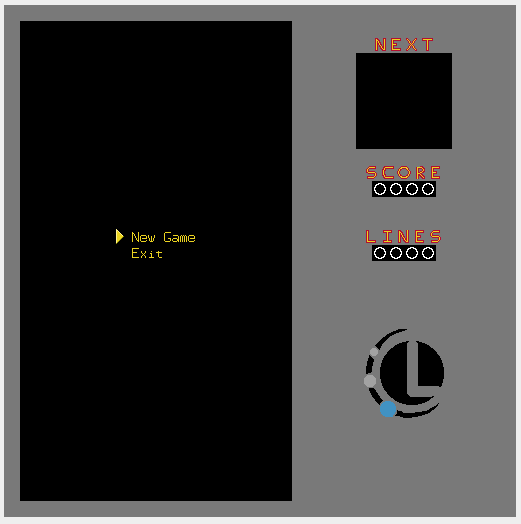
\includegraphics[width=0.65\textwidth]{images/BaseInterface.png} % Include the image placeholder.png
    \caption{Interface inicial do jogo.}
    \label{BaseInterface}
  \end{center}
\end{figure}

O jogo pussui na sua interface(Figura \ref{BaseInterface}) o espaço para o jogo contendo 272 pixels de largura. Uma caixa para exibir a próxima peça que será lançada na tela. Duas caixas pequenas para exibir a quantidade de linhas completadas e a pontuação do jogador.

\begin{figure}[H]
  \begin{center}
    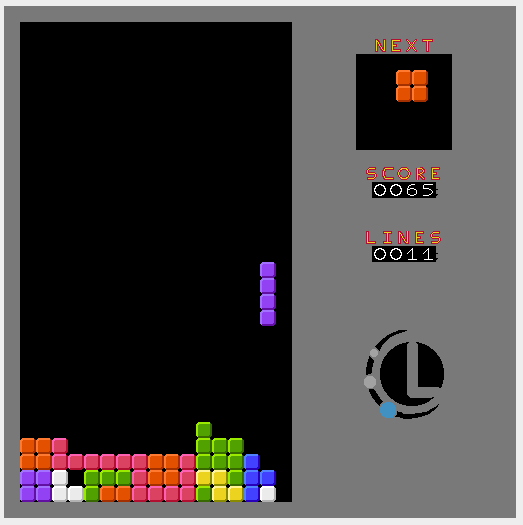
\includegraphics[width=0.65\textwidth]{images/InGame.png} % Include the image placeholder.png
    \caption{Jogo em execução.}
    \label{InGame}
  \end{center}
\end{figure}

As peças podem se mover livremente para esquerda, direita, baixo, e girar dentro do espaço da tela, desde que haja espaço livre.
De tempo em tempo a peça descerá automaticamente, caso não seja possível descer a peça será fixada na tela, linhas completas serão removidas, a pontuação e contador de linhas atualizadas e uma nova peça lançada na tela(Figura \ref{InGame}).

\begin{figure}[H]
  \begin{center}
    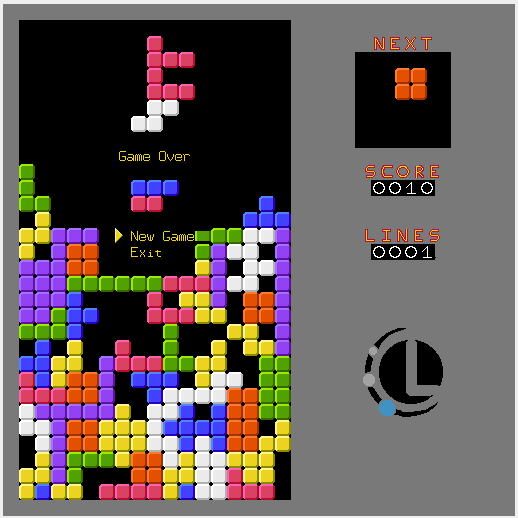
\includegraphics[width=0.65\textwidth]{images/GameOver.png} % Include the image placeholder.png
    \caption{Tela de \textit{Game Over}.}
    \label{GameOver}
  \end{center}
\end{figure}

Caso uma nova peça não possa ser lançada em jogo, a mensagem de \textit{Game Over} aparecera juntamente ao Menu(Figura \ref{GameOver}).

Para jogar o jogo é necessário iniciar MARS carregar o arquivo nomeado \textbf{Main.asm}. Abrir a ferramenta \textit{Keyboard and Display MMIO Simulator}. Abrir a ferramenta \textit{Bitmap Display}, configurar para 512x512 com pixels 1x1, ou, 1024x1024 com pixels 2x2, selecionar endereço base para $\$gp$. Montar o código, conectar as ferramentas ao MARS e lançar a execução em velocidade máxima.

Curiosidades
\begin{itemize}
  \item O jogo pussui um \textit{Ester Egg} que pode ser ativado no Menu inicial ao se digitar $J$ ou $B$.
  \item As paletas de cores utilizadas no jogo pertecem ao conjunto de cores do SNES.
  \item O sistema de potuação do jogo da pontuações maiores quando a linha base é completada
\end{itemize}

\end{document}
